% !TeX root = scaffold-50.tex
\renewcommand{\imagepath}{../50-unsupervised/img}
\newcommand{\ntopics}{n_\text{topics}}
\newcommand{\nclusters}{n_\text{clusters}}

\chapter{Unsupervised Analysis: Topic Modelling}\label{ch:unsupervised}
In this chapter, the topics of the celebrity newspaper articles are examined using the topic modelling technique. After showing that using \gls{lda} alone does not yield robust and reliable results, semantic-similarity clustering is shown to improve the quality of the topic extraction.  Finally, the significance of differences in the topic distributions of low-\gls{ses} and high-\gls{ses} newspaper articles are discussed.

The main focus is to find the prevailing topics in the celebrity newspaper articles and to examine any differences in the distribution of these topics between the low-\gls{ses} and high-\gls{ses} groups.\todo{Motivate more again}

\section{Shortcomings of LDA Topic Modelling}
In a first attempt, \gls{lda} model instances (see chapter~\ref{ch:lda}) were trained for a varying number of topics $\ntopics$. The corpus of all relevant newspaper articles comprised the 50-article balanced data set ensuring that role models with many articles could not induce a topic bias in the models. The texts were fed to the models in the \textit{noun and verb} stage in order to focus on the meaning-bearing elements of the texts.

Each of these model instances yielded a set of $\ntopics$ topics. Each topic $t$ is defined by a list $T_{\ntopics, t}$ of characterizing topic words. Each model assigned to every newspaper article $i$ estimated probabilities $p_{i, t}$ that article $i$ would belong to the topic $t$. Each newspaper article $i$ was assigned a topic $t_i$ by selecting the topic with the maximum probability:
\begin{align}
    t_i = \arg \max_{t'} p_{i, t'}
\end{align}

Figure~\ref{fig:topic_modelling_schema} illustrates the modelling and assigment process.
\begin{figure}
    \centering
    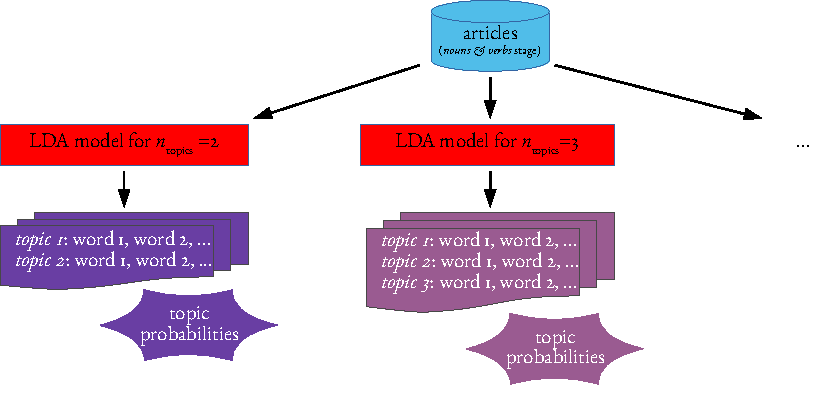
\includegraphics[]{\imagepath/topic_modelling_schema.pdf}
    \caption{Schematic of the topic modelling setup with \gls{lda}: Many models for different numbers $\ntopics$ of topics are trained, each of them yields a list of topics that are characterized by topic words, as well as topic probabilities for each article.}\label{fig:topic_modelling_schema}
\end{figure}

The \gls{lda} algorithm depends on a set of hyperparameters, most of which are related to its underlying optimization process.  Sensible values for these were found by trial and error. The one hyperparameter that is crucial for the interpretation of this analysis is $\ntopics$. It determines the granularity of the topics the model provides for the comparison of the low- and high-\gls{ses} groups. The trade-off between a low and a high number of topics is expected to be a well-graspable set of topics with considerable overlaps and therefore poor specificity for low $\ntopics$, in contrast to highly delimited niche-topics suffering from a lack of generality for high $\ntopics$. For choosing an appropriate $\ntopics$ in this work, it was required that the topics assigned to articles be consistent for small variations of $\ntopics$. Otherwise it could be assumed that the assignment of topics to the articles is to a large part random, which would imply that the findings about the distribution of these topics across the low- and high-\gls{ses} groups is also random. The search for an optimal number of topics included introducing of so-called \textit{hypertopics} to make the topics comparable as well as assessing ranges for $\ntopics$ within which the hypertopic accuracy and the \gls{ses} assignment were consistent:

\paragraph{Assigning Hypertopics}
As the model output topics are only defined by a list of characterizing words, the individual topics can overlap in term of their meaning (e.g. different kinds of sport), and the topics obtained for different $\ntopics$ cannot be compared without human intuition. In order to still be able to compare the model outputs for different $\ntopics$, each topic was manually assigned one of the four \textit{hypertopics} movie, music, sport, and life (with life being intended as a miscellaneous category for all topics not covered by the other three hypertopics). These four hypertopics were heuristically selected while examining the model output topics. Each article $i$ with topic $t$ was assigned a hypertopic $h$:
\begin{align}
    h_i = h(t_i)
\end{align}
Table~\ref{tab:hypertopics} shows examples of the model output topics and their manually assigned hypertopics and shows the generality vs specificity trade-off in terms of the chosen $\ntopics$.

\begin{table}
    \centering
    \begin{tabular}{clc}
        \toprule
        $\ntopics$ & topic words for exemplary topics (model output) & hypertopic \\
        \toprule 
        \multirow{3}{*}{5} & love video fan people thing song feel music share life & \textit{life}\\
        & game player team season goal win league sport club score & \textit{sport}\\
        & film llc st ave dr series movie season actor michael & \textit{movie}\\
        \midrule
        \multirow{3}{*}{50} & music artist business sony continue record label company team partner & \textit{music} \\
        & inc property water art road town science management development site & \textit{life} \\
        & fc week injury season run football quarter marcel yard dortmund & \textit{sport} \\
        \bottomrule
    \end{tabular}
    \caption{Example of model output topics and their respective hypertopics. Comparing the \textit{sport} hypertopic examples for $\ntopics = 5$ and $\ntopics = 50$ shows how a larger amount of model topics makes the topics more specific, here by referencing a particular sport and a particular sports club.}\label{tab:hypertopics}
\end{table}

With every article associated to a hypertopic, it was possible to compare the distribution of articles and \gls{ses} groups across hypertopics for different $\ntopics$, as well as to verify how accurately the topic models had assigned topics to the articles using the human-annotated data.

\paragraph{Accuracy and Consistency}
The accuracy of the hypertopic assignment was calculated as the ratio of articles with correct hypertopic assignment by the model and all articles that were human-annotated:
\begin{align}
    acc = \frac{
        \left|
            \left\{i\middle|h_{i}^\text{predicted} = h_{i}^\text{true}\right\}
        \right|
    }{
        \left|
            \{{i|i \text{ was human-annotated}}\}
        \right|
    }
\end{align}

Figure~\ref{fig:lda_accuracy_diagram} shows that the accuracy greatly depends on $\ntopics$ with a maximum of abount \SI{50}{\percent} at $\ntopics=15$.

\begin{figure}
    \centering
    \begin{pgfpicture}
        \pgftext{../../../build/thesis/50-unsupervised/lda_accuracy_diagram.pgf}
    \end{pgfpicture}
    \caption{Accuracy of the model-assigned hypertopics compared to human-annotated data as a function of the number of topics: A maximum accuracy of around \SI{50}{\percent} was achieved for $\ntopics=15$.The accuracy not consistent across the different numbers of topics.}\label{fig:lda_accuracy_diagram}
\end{figure}

Additionally, the share of low-\gls{ses} articles for each assigned hypertopic was used as a measure for topic assignment consistency across $\ntopics$. This share is plotted in figure~\ref{fig:lda_hypertopic_consistency_diagram}. The fact that there is no range of $\ntopics$ where this share is consistent for small variations of $\ntopics$ suggests that the assignment of articles to the hypertopics is to a considerable extent random and that the model is incapable of making a reliable prediction of an article's topic.\todo{Explain more why you took exactly this share and not anything else.} These observations did not differ significantly if the \textit{distinct-\gls{ses}} set of articles was used instead.

\begin{figure}
    \centering
    \begin{pgfpicture}
        \pgftext{../../../build/thesis/50-unsupervised/lda_hypertopic_consistency_diagram.pgf}
    \end{pgfpicture}
    \caption{Share of low-\gls{ses} articles in each hypertopic across different numbers of topics as an indicator of topic assignment consistency: The share varies substantially over a range from \SI{5}{} to \SI{50}{} topics, indicating that the assigment of articles to topics is not very reliable and not consistent. The share of low-\gls{ses} articles among all articles is shown as a reference.}\label{fig:lda_hypertopic_consistency_diagram}
\end{figure}

Two potential approaches for improving accuracy and consistency were examined: Firstly, it was attempted to train the topic models on the low-\gls{ses} and high-\gls{ses} corpora separately, which, however, led to similar inconsistencies. Secondly, it was tried to filter out articles for which the model's topic assignment was ambiguous. As a measure for the ambiguity in topic assignment for article $i$ with topic probabilities $p_{i, t}$, the information theoretical entropy was used~\autocite{gray_entropy_2013}:
\begin{align}
    H_i = \sum_t p_{i, t} \ln p_{i,t}
\end{align}
The entropy is low if the probability distribution clearly favors a specific topic, and it is high if the probabilities $p_{i, t}$ are rather ambiguous. After filtering out articles where $H_i$ is higher than the \SI{50}{\percent}- or \SI{30}{\percent}-percentile of all articles, higher accuracies of up to \SI{70}{\percent} were reached, however the consistency problem persisted and due to filtering out articles some hypertopics were not present in the remaining set of articles in some cases. The topic modelling quality could hence not be substantially improved by these measures.

The author guesses that one of the reasons for the inconsistent variations in topic assignment is the newspaper articles operate on a very limited set of topics, roughly covered by the four hypertopics, which do expose considerable overlaps (e.g. movie-related articles having similarity to life stories, film music-related articles talking about movies). This could render the topic models incapable of capturing distinct groups of articles, rather than assigning topics seemingly at random.

As the quality of the topic modelling approach could not be substantially improved without the scope of \gls{lda}, the modelling process was enhanced by adding pretained transformer model providing semantic embeddings as described in the next section.

\section{Improvement with a Pretrained Model}
In order to mitigate the issue that the \gls{lda} topic model was apparently incapable of consistenly separating articles by their meaning, a pretrained semantic embedding model was added to the modelling process. It was used assign to every newspaper article a vector representation of its meaning (semantics) that could be partitioned into topics by a clustering algorithm:

As a first step, each article in the \textit{content} stage, meaning the original article with only minimal cleaning applied, was assigned a $384$ dimensional vector representation by the pretrained SentenceBERT model (implemention with \textcite{sbertsentencetransformers_sentencetransformers_2022}, see chapter~\ref{ch:sentencebert}). As suggested by \textcite{black_using_2020}, these representations were first dimensionality-reduced to \SI{50}{} dimensions using \gls{pca}~\autocite{pearson_liii_1901} and then further reduced to \SI{3}{} dimensions using \gls{tsne}~\autocite{maaten_visualizing_2008}. This procedure yielded a three-dimensional semantic vector representation of each article, such that articles with similar meaning are closer to each other in this vector space than articles with a large difference in meaning.

In the next step, these vectors were then used as input for the KMeans clustering algorithm~\autocite{1967} for partitioning the articles according to their meaning, such that articles with similar meaning are rather within the same cluster whereas articles with differing meaning are more likely to be in different clusters. This algorithm produced $\nclusters$ clusters, each one representing one topic. Figure~\ref{fig:clusters} shows the articles' vector representation and the clusters for $\nclusters=5$ in two dimensions. In this way, the process of assigning topics to each article did not depend on the newspaper article corpus anymore but instead on a pretrained model.

Finally \gls{lda} with $\ntopics=1$ was applied on the articles of each cluster in the \textit{nouns and verbs} stage, hence with most of the structure removed from the text. In this way, each cluster was assigned a single set of topic words, such that in the end the output of the modelling process had the same structure as for using \gls{lda}.

Figure~\ref{fig:embedding_modelling_schema} illustrates this modelling procedure from the articles, over the vector representations, to the clusters representing topics. In figure~

\begin{figure}
    \centering
    \includegraphics[]{\imagepath/cluster_diagram.pdf}
    \caption{Two-dimensional representation of the vector embeddings of the newspaper articles. The different colors denote the different clusters found by the KMeans algorithm. The clusters may seem to be incontiguous because the clustering was performed on the three-dimensional data whereas this representation is two-dimensional. Note that the two axes have no intuitive meaning, they represent the two main components of the original SentenceBERT embedding of each article.}\label{fig:clusters}
\end{figure}

\begin{figure}
    \centering
    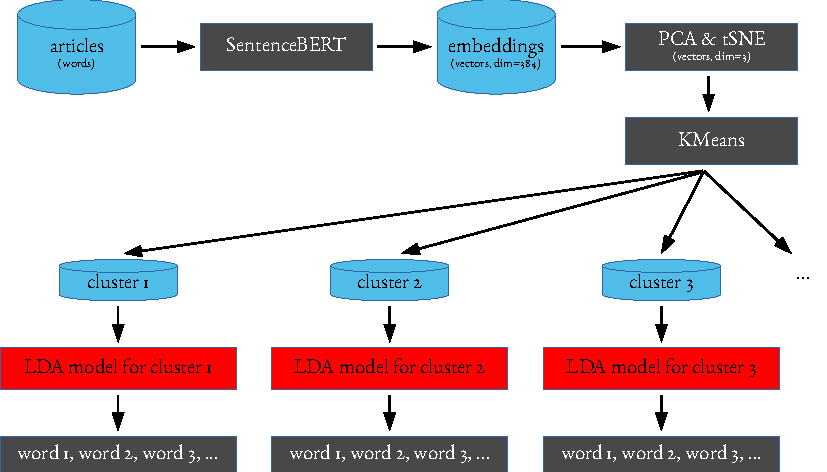
\includegraphics[]{\imagepath/embedding_modelling_schema.pdf}
    \caption{Schematic of the topic modelling process with SentenceBERT semantic embeddings and KMeans clustering: The article texts (in the \textit{content} stage) are transformed into embeddings, a vector representation of text, by the pretrained SentenceBERT transformer model. These representations are dimensionality-reduced with \gls{pca} and \gls{tsne}. Then the KMeans algorithm clusters the articles into $\nclusters$ clusters. Each of these sets of articles represents a topic whose topic words are found by separate \gls{lda} models (with $\ntopics=1$, taking the articles in the \textit{nouns and verbs} stage as input) for each cluster.}\label{fig:embedding_modelling_schema}
\end{figure}

\paragraph{Accuracy and Consistency}
Again, hypertopics were assigned to each set of topic words for evaluating the accuracy and assessing consistency across $\nclusters$. With this enhanced approach, higher accuracies of up to \SI{75}{\percent} and more consistency in topic assignment was achieved, as can be seend from figures~\ref{fig:semantic_clustering_accuracy_diagram} and~\ref{fig:semantic_clustering_hypertopic_consistency_diagram}.

\begin{figure}
    \centering
    %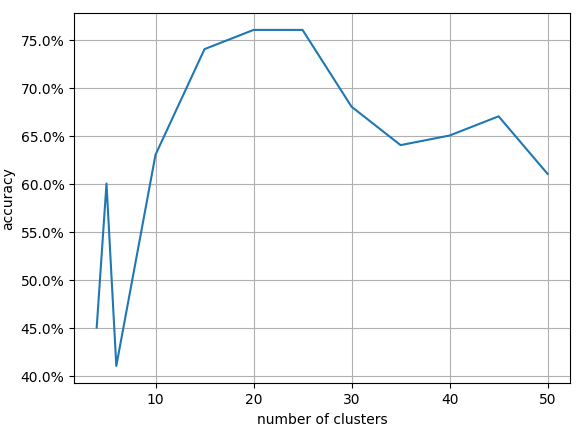
\includegraphics[scale=0.5]{\imagepath/acc_by_n_embeddings.png}
    \begin{pgfpicture}
        \pgftext{../../../build/thesis/50-unsupervised/semantic_clustering_accuracy_diagram.pgf}
    \end{pgfpicture}
    \caption{Accuracy of the  enhanced model-assigned hypertopics compared to human-annotated data as a function of the number of topics: The accuracy is higher and more consistent across the different numbers of clusters compared to the \gls{lda} approach. A value of $\nclusters=20$ seems promising.}\label{fig:semantic_clustering_accuracy_diagram}
\end{figure}

\begin{figure}
    \centering
    % 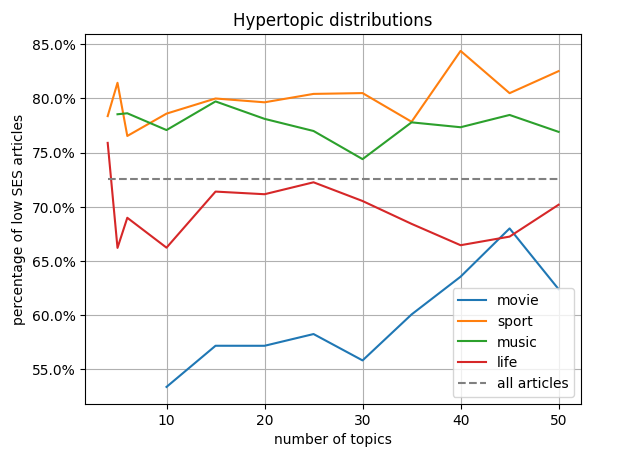
\includegraphics[scale=0.5]{\imagepath/low_ses_by_n_embeddings.png}
    \begin{pgfpicture}
        \pgftext{../../../build/thesis/50-unsupervised/semantic_clustering_hypertopic_consistency_diagram.pgf}
    \end{pgfpicture}
    \caption{Share of low-\gls{ses} articles in each hypertopic across different numbers of topics: The share is comparably consistent around $\nclusters=20$ for all hypertopics, making it a promising choice. The share of low-\gls{ses} articles among all articles is shown as a reference.}\label{fig:semantic_clustering_hypertopic_consistency_diagram}
\end{figure}

As the highest accuracy was achieved for a value of $\nclusters=20$ with comparably little variation around it, this choice was kept for the following analysis. Figure~\ref{fig:embedding_confusion_matrix} compares the hypertopics assigned by the model and the human-annotated hypertopics. It shows that the overall performance of the model is good, however some of the articles that the human annotator had labelled as \textit{movie} or \textit{music} were classified as \textit{life}. This is not surprising considering that celebrity reports do often also cover celebrities' lifestories to a significant extent. For the \textit{distinct-SES} approach, somewhat less accuracy is achieved, the predictions appear, however, equally consistent.

\begin{figure}
    \centering
    \includegraphics[]{\imagepath/semantic_clustering_confusion_matrix.pdf}
    \caption{Confusion matrix of the hypertopics for $\nclusters=20$:}\label{fig:embedding_confusion_matrix}
\end{figure}

\paragraph{Evaluation}
The distribution of articles across the \SI{20}{} topics was compared between the low- and high-\gls{ses} groups in order to identify any significant differences in prevalence of and thus potentially preference for certain topics in the groups' respective celebrity news consumption.

The distribution of the hypertopics for the \textit{general} and the \textit{distinct-SES} approaches is shown in figure~\ref{fig:semantic_clustering_hypertopic_distribution}. The distribution of all \SI{20}{} topics and their respective topic words is presented in figure~\ref{fig:semantic_clustering_cluster_distribution} the appedix chapter~\ref{ch:unsupervised_appendix}.

\begin{figure}
    \centering
    \begin{subfigure}{0.48\textwidth}
        \centering
        \begin{pgfpicture}
            \pgftext{../../../build/thesis/50-unsupervised/semantic_clustering_hypertopic_distribution.pgf}
        \end{pgfpicture}
        \caption{\textit{general} approach}
    \end{subfigure}
    \begin{subfigure}{0.48\textwidth}
        \centering
        \begin{pgfpicture}
            \pgftext{../../presentation/img/semantic_clustering_hypertopic_distribution_distinct.pgf}
        \end{pgfpicture}
        \caption{\textit{distinct-\gls{ses}} approach}
    \end{subfigure}
    \caption{Distribution of articles across hypertopics for the low- and the high-\gls{ses} groups; left for the \textit{general}, right for the \textit{distinct-SES} approach. While the \textit{life} hypertopic is equally represented in both \gls{ses} groups, \textit{movie}-related articles are more prevalent in the high- than in the low-\gls{ses} group, whereas \textit{music} and \textit{sport}-related articles more in the low-\gls{ses} than in the high-\gls{ses} group}\label{fig:semantic_clustering_hypertopic_distribution}
\end{figure}

The graphs reveal that the topic \textit{movie} is more prevalent in the high-\gls{ses} group compared to the low-\gls{ses} group, whereas the topics \textit{music} and \textit{sport} are more represented in the low-\gls{ses} than in the high-\gls{ses} group. For the all-encompassing \textit{life} hypertopic, the groups show only little difference.

In order to estimate the significance of these differences in the topic distributions, two types of $\chi^2$-tests were performed:
\begin{itemize}
    \item An overall $\chi^2$-contingency test assessed whether it the distribution of articles across topics is different for low- and high-\gls{ses}~\autocite[p. 430]{fahrmeir_spezielle_2016}:
    \begin{align}
        \begin{split}
            H_{0, \text{contingency}}: ~~~ &\text{distributions } p_{s, t} \text{ over topics } t \text{ are indepedent of } s\\
        & \text{i.e. } p_{s, t} = p_s \cdot p_t ~~ \forall t, s
        \end{split}
    \end{align}
    with the relative frequencies of articles $p_s$ per \gls{ses}, $p_t$ per topic, and $p_{s, t}$ per \gls{ses} and topic. Rejecting $H_0$ means that both the topic distribution is different for low- and high-\gls{ses}.

    \item A second set of $\chi^2$ tests was performed per topic $t$, assessing whether the respective amount of low- and high-\gls{ses} articles in that topic equals the expected number over all topics:
    \begin{align}
        \begin{split}
            H_{0, \text{ topic }t}: ~~~ &\text{number of articles } n_{s, t} \text{ equals expected number } \tilde n_{s, t} \\
            & \text{i.e. } n_{\text{low}, t} = \tilde n_{\text{low}, t} \text{ and } n_{\text{high}, t} = \tilde n_{\text{high}, t}
        \end{split}
    \end{align}
    $\tilde n_{s, t}$ is the expected number of articles per topic under the assumption of an equal percentage of articles in topic $t$ in both \gls{ses} groups:
    \begin{align}
        \tilde n_{s, t} = n_s \cdot \frac{n_t}{n}
    \end{align}
    $n_s$ is the number of articles in \gls{ses} group $s$, $n_t$ the number of articles in topic $t$, and $n$ the total number of articles. Rejecting $H_0$ means that 
\end{itemize}

Both kinds of $\chi^2$-tests were conducted using the respective functions in the \textit{scipy} library \autocite{scipychi2_scipy_nodate,scipychi2_contingency_scipy_nodate}.

Table~\ref{tab:embeddings_hypertopics_chi2s} shows that...

\begin{table}
    \centering
    ../../../build/thesis/50-unsupervised/semantic_clustering_hypertopic_chi2_table.tex
    \caption{Results of the $\chi^2$-contingency and topic-wise tests for the hypertopics: \todo[inline]{describe results}}\label{tab:embeddings_hypertopics_chi2s}
\end{table}

\paragraph{Alternative Approach: Adjectives and Adverbs}


\section{Discussion}
In this chapter, topic modelling was explored as 